\documentclass[]{seti2}

 \usepackage{wrapfig}% embedding figures/tables in text (i.e., Galileo style)
 \usepackage{threeparttable}% tables with footnotes
 \usepackage{dcolumn}% decimal-aligned tabular math columns
  \newcolumntype{d}{D{.}{.}{-1}}
 \usepackage{nomencl}% automatic nomenclature generation via makeindex
% \usepackage{subfigure}% subcaptions for subfigures
% \usepackage{subfigmat}% matrices of similar subfigures, aka small mulitples
 \usepackage{fancyvrb}% extended verbatim environments
 \usepackage{amsmath}
 \usepackage{placeins}
% \usepackage{subfig}
 \usepackage{setspace}
 \usepackage[justification=centering]{caption}
 \usepackage{graphicx}
 \usepackage[justification=centering]{subcaption}
% \usepackage{cite}
% \usepackage{natbib}
  \fvset{fontsize=\footnotesize,xleftmargin=2em}
	\usepackage{lettrine}% dropped capital at beginning of paragraph
	\usepackage[dvipost]{dropping}% alternative dropped capital package
	%\usepackage{hyperref}% embedding hyperlinks [must be loaded after dropping]
	\usepackage[utf8]{inputenc}
	\usepackage{color}
	\usepackage{graphicx}
	\usepackage{epstopdf}
	\usepackage[english]{babel}
	
 \title{\uppercase{Simulation of Shunt Active Filter for Aircraft Electrical System}}

 \author{
					João Paulo de Souza Olivera\\
					{\normalsize\itshape Área Temática: Sistemas}\\
%					\and
%					Frederico Simões\\
%					{\normalsize\itshape Área Temática: Aeronáutica}\\
%					\and
%					Pedro Ciloni\\
%					{\normalsize\itshape Área Temática: Aeronáutica\footnote{\scriptsize{A lista completa de áreas temáticas está apresentada no site: \textcolor[rgb]{0,0,1}{http://eng.embraer.com.br/SETI}}}}\\
				}

\begin{document}

%Título do documento:
\maketitle

%Resumo:
%=============================================================================================
\begin{abstract}
		\underline{\textbf{Abstract}}: The power quality in aircraft electrical systems became an important issue due to the continuous expansion of electrical loads connected to the distribution system. This study focuses on the power quality improvement and power factor correction by the utilization of active filtering connected at the terminals of non-linear loads. A simulation is proposed with a shunt active filter connected at the power input of an electrohydraulic actuator operating in an electrical grid. The results obtained comprise the system voltages waveforms within the aeronautical standard MIL-STD 704F constraints for distortion factor and distortion spectrum.
\end{abstract}

\textbf{\textit{Palavras-Chave: Power Quality, THD, Active Filter}}

\section{Introduction}

The increase of the aircraft operational costs associated with the fuel consumption drives the development of new aircraft technologies \citep{Babikian2002}. In this scenario, the aviation market has changed the design perception regarding the electrical system, replacing hydraulic and pneumatic’s power source to equivalent electrical ones, creating the concept of the More Electrical Aircraft (MEA) \citep{Moir1999}.

This context raised the relevance of the EPGDS (Electrical Power Generation and Distribution System) in the role of aircraft operational safety. Thus, the electrical system needs to have a greater reliability and operates in such a way to avoid failures of the equipment connected to the grid. However, the increase of the amount of non-linear loads has raised the harmonic distortion content introduced in the EPGDS \citep{Singer2012}, diminishing the power quality and becoming a subject of study in aircraft operational safety. 

To improve the power quality with the reduction of the total harmonic distortion (THD), some conditioners must be connected in the equipment power input and/or in the distribution grid. The implementation of these conditioners must consider the reliability, weight and cost to be feasible in aircraft design.

In this context, some topologies to increase the power quality are already used in the aircraft electrical system, such as the multi-pulse rectifiers \citep{Zhu2014,Gong2003,Lobo2005}. However, its weight and volume make this topology applicable only to specific equipment.

With the increase of the non-linear loads applied to the electrical grid, along with the requirements to ensure power quality, some alternatives of power factor correction have been proposed. In this scenario, the use of a shunt active filter applied in an aircraft is an item of recent study, considering different active filters topologies \citep{Chen2012research,Chen2012novel,Chen2012control}.

This article analyses the use of a shunt active filter to improve the power quality in the aircraft EPGDS. It starts by reviewing the active filter operation, the instantaneous power theory, and continues discussing control techniques. A simulation is presented to analyze the shunt active filter operation with three electrohydraulic actuators (EHA), which are non-linear loads used to control the aircraft latero-directional and longitudinal aerodynamics surfaces. The simulation model is compounded by the electrical generation and distribution system connected to EHAs with their respective shunt active filters.


\section{Power Quality in Aircraft}\label{sec:Power_Quality}

The power quality in aircraft EPGDS is a concern which regards the airworthiness. The electrical equipment used in aircraft design must be qualified to ensure the proper operation and integration. Thereby, the power quality is one of the subjects considered in the qualification tests, which are specified by standard test procedures issued by aeronautical authorities. The most used qualifications standards for electrical systems are the MIL-STD 704, which qualifies the EPGDS, and the DO-160 - Section 16, which qualifies the embedded electrical equipment. To ensure the proper equipment integration, the EPGDS  and equipment must comply with these standards.

The non-linear loads inject harmonic distortion content in the system, inducing degradation in the power quality and decreasing the power factor. Furthermore, the increase in the number of electrical equipment connected in the grid enhances the degradation of the power quality. Thus, techniques for power factor correction must be applied in the EPGDS to limit the system operation within the constraints of aeronautical standards.

Some techniques are already used in aircraft electrical system to increase the power factor and power quality. One of these techniques is the use of multi-pulse converters, which is most employed in high capacity loads rectifiers to improve the power quality. However, despite of the good reliability, they are bulky and heavy. There are some other topologies that are useful for harmonic content reduction, but their characteristics do not make them feasible to operate in the aircraft systems. Some of these topologies are the passive filters and power factor correction (PFC) converters. For the passive filters, despite of good reliability and low cost, the high weight is the main problem to its implementation in aircraft \citep{Barruel2004}. For the PFC converters, the downside lies in the low reliability and low density of energy conditioned \citep{Zhu2014,Gong2003,Lobo2005}. 

In this scenario, the active filter, due to its features as lightweight and fast response to load variation, appears to be a feasible topology to reduce the harmonic content and increase the power factor \citep{Zhu2014,Chen2012control,Karatzaferis2013}. There are some drawbacks in its use, as the high complexity and low reliability, but the advances in power electronics are making them practical to be implemented in aircraft electrical system \citep{Abdelhafez2009}.







\section{Active Filters}

The active filter operates creating waveforms to interact with the voltages and currents presented in the electrical grid to establish a power factor equal to one. This is accomplished by measuring the voltage waveforms from the power source and the current waveforms from the load, and then using these parameters on the instantaneous power theory to determine the current reference as an input to be set in a compensator. The compensator injects current waveforms in the circuit with symmetrical values of the components which degrades the power factor. The typical system compounded by a non-linear load with an active filter is presented in Fig. \ref{fig:compensador.png}.

\begin{figure}[!h]
\centering
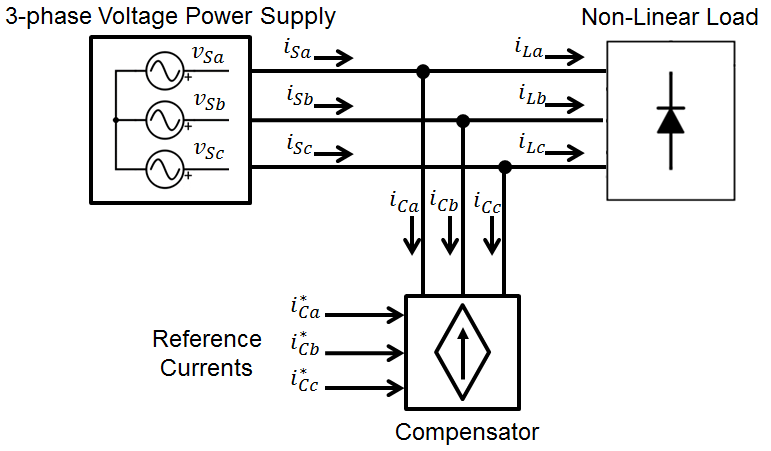
\includegraphics[width=2.8in]{Figures/compensador.png}
\caption{Simulation Results}
\label{fig:compensador.png}
\end{figure}

%\begin{figure}
%	\centering
%	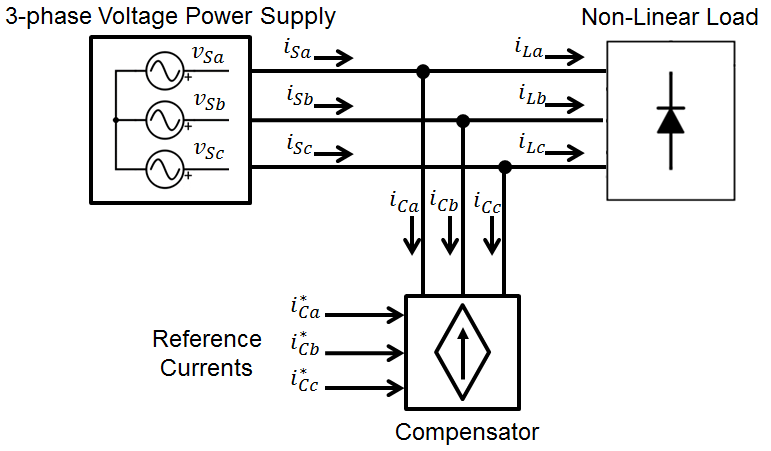
\includegraphics[width=0.4\textwidth]{Figures/compensador.png}
%	\caption{Simulation Results}
%	\label{fig:compensador.png}
%\end{figure}


\subsection{Instantaneous Power Theory}

The instantaneous power theory was presented by Akagi \cite{Akagi}, which proposed some new concepts for the instantaneous active and reactive power. This theory can be used in three phase, three or four wire system and in steady or transient state \cite{Akagi,Akagi}. In this theory, the manipulation of the active and reactive power calculations brings a tool to determine the currents that carry some content which degrade the power factor, such as harmonic distortion and phase shift.
Considering a three-phase system, composed by the phases $a$, $b$ and $c$, the instantaneous power theory is based in the coordinates transformation from the $abc$ to $\alpha \beta 0 $. This is known as the Clarke Transformation and is shown in eq. (2) \ref{eq:Clarke}.

\begin{equation}
\begin{aligned}
\begin{bmatrix}
v_0\\
v_\alpha\\
v_\beta
\end{bmatrix}
& = \sqrt{\dfrac{2}{3}}
\begin{bmatrix}
\dfrac{1}{\sqrt{2}}	& \dfrac{1}{\sqrt{2}}	& \dfrac{1}{\sqrt{2}}		\\[2ex]
1					& -\dfrac{1}{2}			& -\dfrac{1}{2}				\\[2ex]
0					& \dfrac{\sqrt{3}}{2}	& -\dfrac{\sqrt{3}}{2}
\end{bmatrix}
\begin{bmatrix}
v_a\\
v_b\\
v_c
\end{bmatrix}
;\\
\begin{bmatrix}
i_0\\
i_\alpha\\
i_\beta
\end{bmatrix}
& = \sqrt{\dfrac{2}{3}}
\begin{bmatrix}
\dfrac{1}{\sqrt{2}}	& \dfrac{1}{\sqrt{2}}	& \dfrac{1}{\sqrt{2}}		\\[2ex]
1					& -\dfrac{1}{2}			& -\dfrac{1}{2}				\\[2ex]
0					& \dfrac{\sqrt{3}}{2}	& -\dfrac{\sqrt{3}}{2}
\end{bmatrix}
\begin{bmatrix}
i_a\\
i_b\\
i_c
\end{bmatrix}
\label{eq:Clarke}
\end{aligned}
\end{equation} 

According to \cite{Akagi}, the instantaneous power is defined as shown in eq (3) \ref{eq:pq_0}, where the $p_0$, $p$ and $q$ are the instantaneous zero-sequence power, the active instantaneous power and the reactive instantaneous power, respectively \cite{Akagi,Peng1996}.

\begin{equation}
\begin{bmatrix}
p_0\\
p\\
q
\end{bmatrix}=
\begin{bmatrix}
v_0		&	0			&	0\\
0		&	v_{\alpha}	&	v_{\beta}\\
0		&	v_{\beta}	&	-v_{\alpha}
\end{bmatrix}
\begin{bmatrix}
i_{0}\\
i_{\alpha}\\
i_{\beta}
\end{bmatrix}
\label{eq:pq_0}
\end{equation} 

Considering a system without zero-sequence voltage and/or current, such as the aircraft electrical system, the eq (3) can be simplified as the eq (4), where the instantaneous zero-sequence power is absent.

\begin{equation}
\begin{bmatrix}
p\\
q
\end{bmatrix}=
\begin{bmatrix}
v_{\alpha}	&	v_{\beta}\\
v_{\beta}	&	-v_{\alpha}
\end{bmatrix}
\begin{bmatrix}
i_{\alpha}\\
i_{\beta}
\end{bmatrix}
\label{eq:pq}
\end{equation} 

The reverse calculation, i.e., the determination of the currents $i_{\alpha}$ and $i_{\beta}$ when the voltages $v_{alpha}$ and $v_{\beta}$ and the instantaneous power $p$ and $q$ are known is presented in eq. (5) \ref{eq:i_alphabeta}.

\begin{equation}
\begin{bmatrix}
i_{\alpha}\\
i_{\beta}
\end{bmatrix}=
\dfrac{1}{v_{\alpha}^2+v_{\beta}^2}
\begin{bmatrix}
v_{\alpha}	&	v_{\beta}\\
v_{\beta}	&	-v_{\alpha}
\end{bmatrix}
\begin{bmatrix}
p\\
q
\end{bmatrix}
\label{eq:i_alphabeta}
\end{equation}

By definition, the active instantaneous power is composed by the energy that is swapped between two subsystems, whereas the reactive power is composed by the energy being swapped between the 3 phases of the system \cite{Akagi}. Furthermore, both $p$ and $q$ can be defined as a composition of an average ($\overline{p}$ and $\overline{q}$) and an oscillating ($\tilde{p}$ and $\tilde{q}$) values, as defined in eq. (6) \ref{eq:pq_m_o}.

\begin{equation}
\begin{aligned}
p = \overline{p} + \tilde{p}\\
q = \overline{q} + \tilde{q} 
\end{aligned}
\label{eq:pq_m_o}
\end{equation} 

To create an active filter to coordinate a power factor equal to 1, the only permitted power flowing in the transmission lines is the average value of the instantaneous active power ($\overline{p}$). To ensure this condition, the filter must inject in the lines currents which contains the symmetrical values of the instantaneous reactive power ($q$) and the oscillating portion of the instantaneous active power ($\tilde{p}$) created by the non-linear load. By doing this, these powers are cancelled in the same way as the current harmonic content. Thereby, the selection of power to be compensate and processed by the filter must contains the values of the $-\tilde{p}$ and $-q$ only.

The filter full operation is defined by the instantaneous power $p$ and $q$ calculation, followed by the selection of the power to be compensated, i.e., $-\tilde{p}$ and $-q$. Afterwards, the currents $i_{\alpha}$ and $i_{\beta}$ are calculated using the eq (5) \ref{eq:i_alphabeta} with the values $-\tilde{p}$ and $-q$, followed by the inverse Clarke transformation to acquire the current in $abc$ coordinates to be applied as a reference in the compensator. The whole active filter reference definition is shown in Fig. \ref{fig:diagrama_filtro.png}.

\begin{figure}[!th]
	\centering
	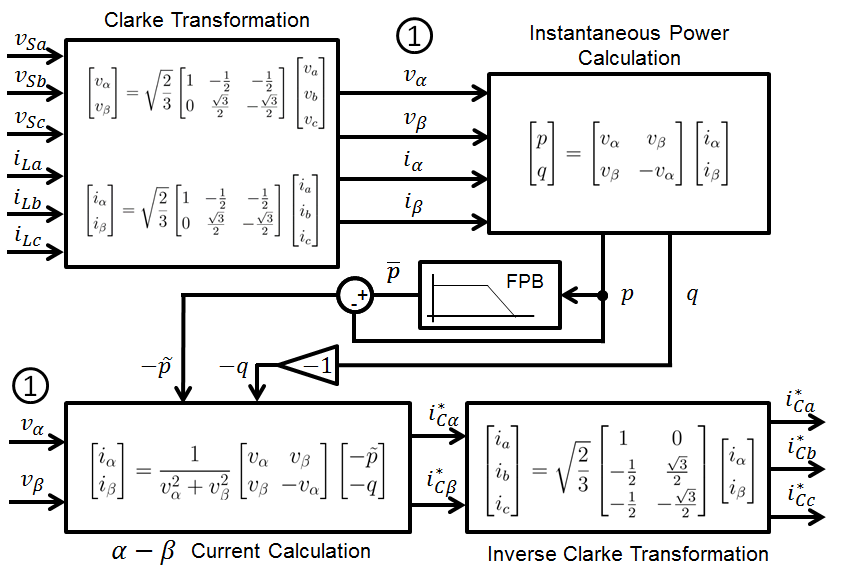
\includegraphics[width=3in]{Figures/diagrama_filtro.png}
	\caption{Simulation Results}
	\label{fig:diagrama_filtro.png}
\end{figure}

%\begin{figure}
%	\centering
%	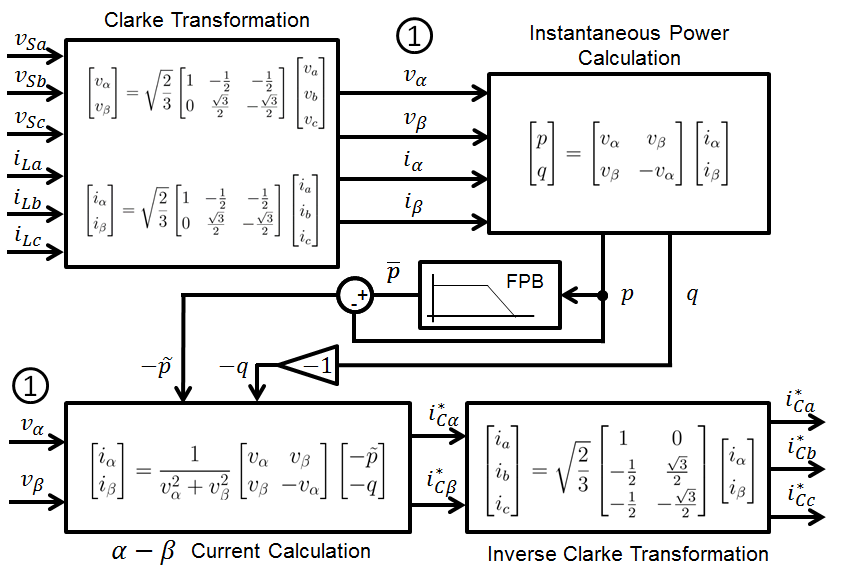
\includegraphics[width=0.47\textwidth]{Figures/diagrama_filtro.png}
%	\caption{Active filter reference definition}
%	\label{fig:diagrama_filtro.png}
%\end{figure}

\subsection{Control Strategy}

The active filter specified in Fig (7) \ref{fig:diagrama_filtro.png} presents very effective to set the current reference to be applied in the compensator for mitigation of the electrical system harmonic content. However, this calculation is valid to produce sinusoidal current waveforms only when the voltages measured and used in the filter input is pure sine waves. This happens since the filter operates in such way that only the mean value of the active instantaneous power flows in the circuit. Therefore, the use of a non-sinusoidal voltage waveform in the input of the filter requires a non-sinusoidal current waveform to establish the power flow with only $\overline{p}$.

In aircraft electrical power system, the voltage waveforms stated in the point of common connection (PCC) are presented as non-sinusoidal, however, they are still limited by the aeronautical standards. As the voltages used in the active filter are measured at the PCC or beyond this point, its operation is not optimal for power quality purposes, and, in some cases, it may decrease the power quality and operates unstably depending the levels of harmonic distortion presented in the voltages waveforms.

According to \cite{Akagi2007}, the p-q theory proves insufficient to satisfy the condition to create a current sine wave and an active instantaneous power flow consisted of only the its mean value, at the same time the voltage waveforms measured and presented on the PCC are previously distorted. To overcome this situation, a control strategy based on the use of a positive-sequence voltage detector is employed to ensure a sinusoidal current control. With this, the power flow between the load and the source is not defined as the mean value of the active instantaneous power, however, the control strategy relays on the appropriate sine wave current insertion in order to establish the proper power quality at the system.

This control is designed by the use of the positive-sequence voltage detector, which operates to extract the fundamental positive-sequence component from the distorted voltages. This component is required by the active filter to define the current shape to be applied in the electrical grid to create a sinusoidal waveform.

The positive-sequence voltage detector operates based on the p-q dual theory where it is used a phase locked loop (PLL) and the p-q theory to extract the fundamental frequency and amplitude of the distorted voltages. The PLL is show in Fig. \ref{fig:PLL.png} and operates defining the fundamental frequency and phase. The scheme shown in Fig. \ref{fig:detector_seq_positiva.png} uses the p-q theory and the information coming from the PLL to define the amplitude of the fundamental component to be used in the active filter calculations.

\begin{figure}[!th]
	\centering
	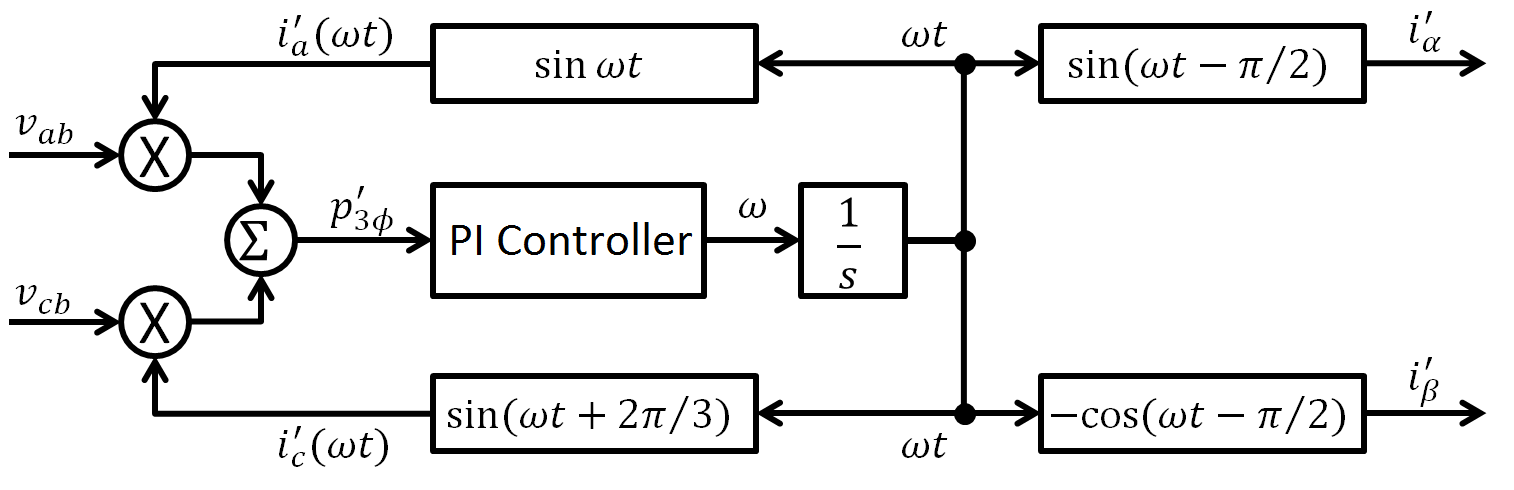
\includegraphics[width=3in]{Figures/PLL.png}
	\caption{Phase locked loop}
	\label{fig:PLL.png}
\end{figure}

\begin{figure}[!th]
	\centering
	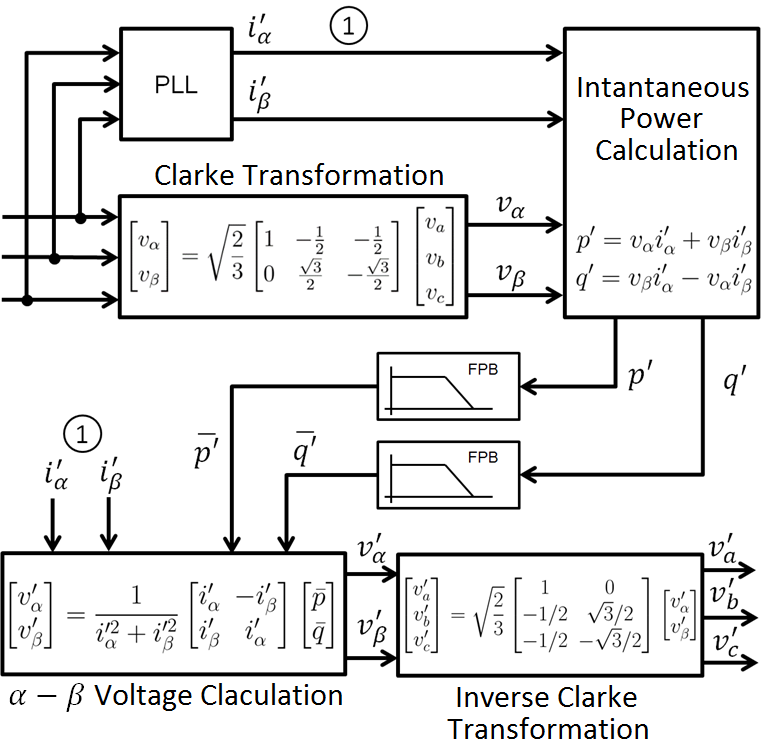
\includegraphics[width=3in]{Figures/detector_seq_positiva.png}
	\caption{Positive-sequence detector}
	\label{fig:detector_seq_positiva.png}
\end{figure}

In the operation of the active filter, some loss is presented in the circuit, mainly due to the VSC switching devices, which cause the voltage of the capacitor, locate in the converter DC side, to decrease. To avoid this voltage drop, a closed-loop design with a PI controller is applied in the active filter to define the power to compensate the system power loss. This closed-loop error signal is processed by the compensator, causing this to manage the power flow in the VSC to hold the capacitor voltage to specifically reference.


\section{Simulation of the Shunt Active Filter Operating with an Electrohidraulic Actuator}

The operation of the shunt active filter in an aircraft electrical system was evaluated by simulation. The system is composed by the generation and distribution system and some loads constituted by electrohydraulic actuators (EHAs) with shunt active filters connected to its respective inputs.

\subsection{Active Filter Model}

The shunt active filter consists of a Current Reference Calculator and a Compensator, as shown in Fig. \ref{fig:filtro_blocos_1.png}. This figure shows these parts with its respective internal sub-blocks. The Current Reference Calculator block is comprised by the Positive Sequence Detector (Fig. 4 \ref{fig:detector_seq_positiva.png}) and the Active Filter Reference Definition (Fig. 2 \ref{fig:diagrama_filtro.png}). These sub-blocks are responsible for the calculation algorithm (each sub-block presents its respective signals inputs and outputs) to determine the reference to be applied in the compensator. The Compensator is presented by the VSC with its respective hysteresis controller and capacitor voltage PI controller. This figure shows also the voltages and currents measurement probes connection in the electrical grid, where acquire the inputs for the active filter operaion.

The reference calculator block defines the proper reference to be applied in the compensator. Its inputs are the load currents and the grid voltages measurements, while its output is the reference applied to the compensator. The compensator block consists of a VSC with its capacitor DC voltage regulated by a closed-loop controller. The compensator also has the hysteresis controller, which creates the commands applied to the VSC switching devices.

The shunt active filter operation requires a passive capacitor filter applied in the transmission lines to eliminate the high frequency content injected in the system by the switching commutation \cite{Akagi2007}. Due to high switching commutation frequency, the passive filter is lightweight and does not impact significantly in the aircraft system. However, the presence of capacitors in the transmission lines may decrease the power factor due to current phase shift. To eliminate this, inductors may be applied in the lines to compensate the reactive power flow.

\begin{figure*}[!tb] %
	\centering
	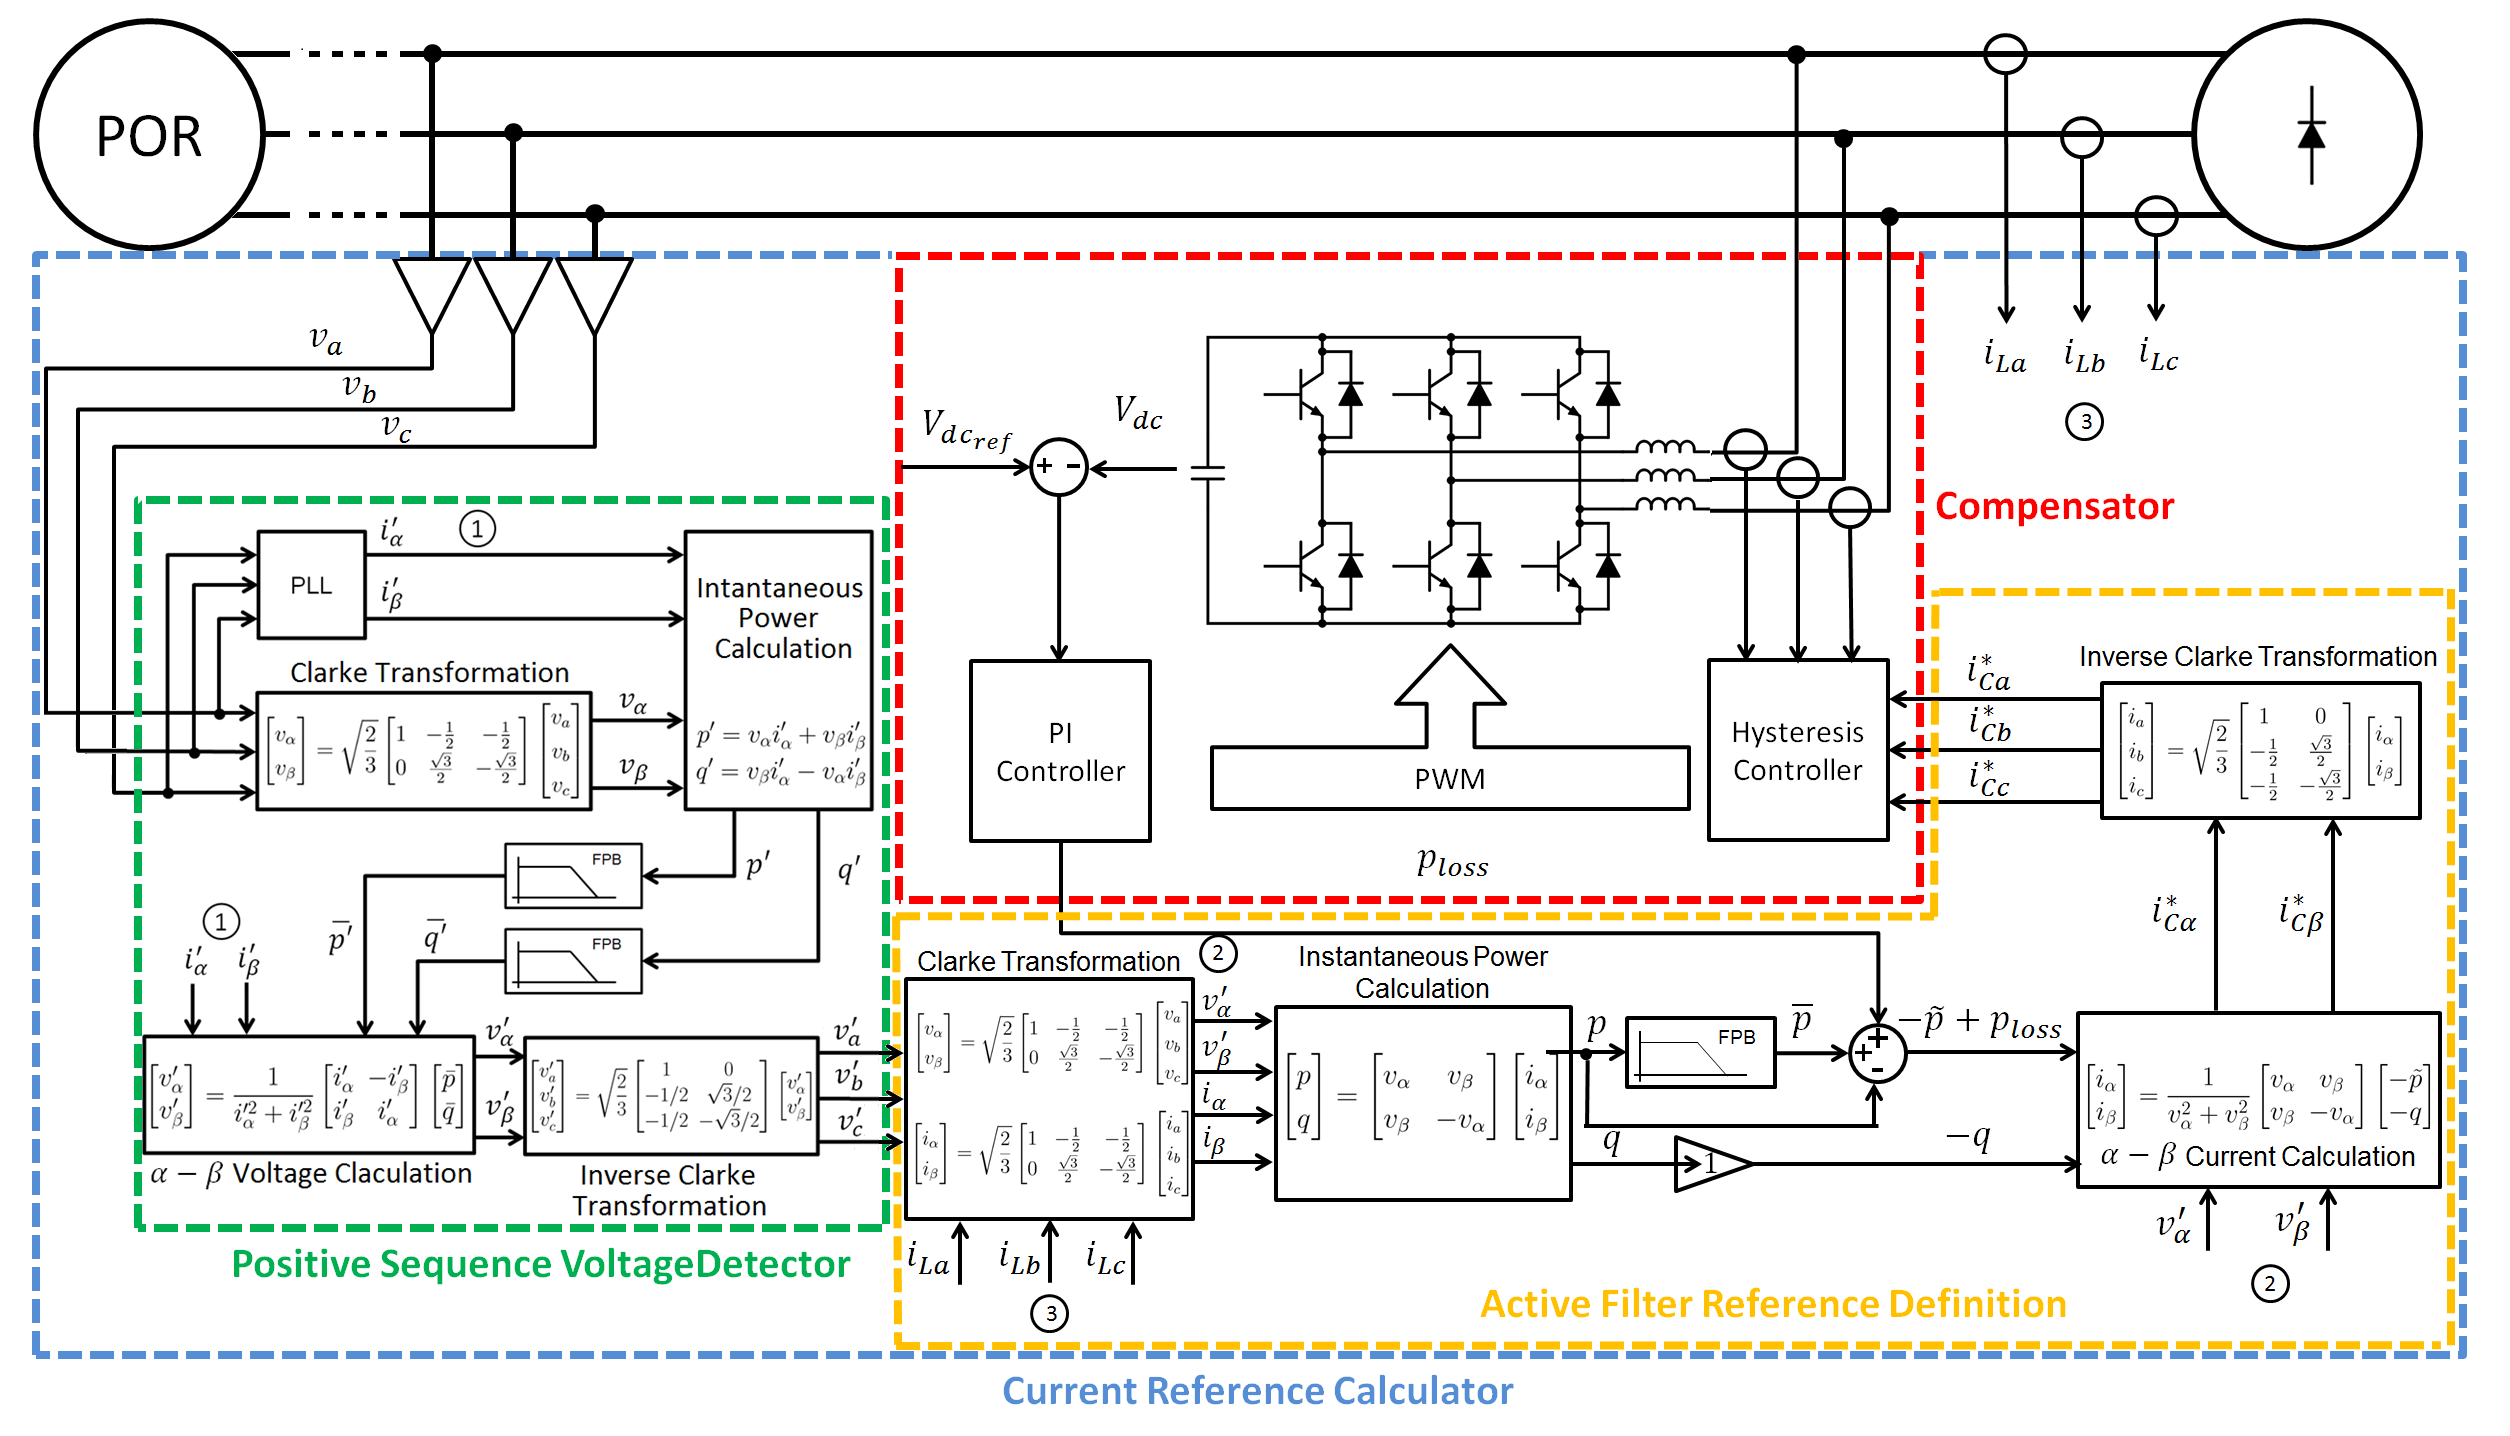
\includegraphics[width=0.83\textwidth]{Figures/filtro_blocos_1.png}
	\caption{Shunt active filter scheme}
	\label{fig:filtro_blocos_1.png}
\end{figure*}

\subsection{Electrical System Model}

The aircraft electrical system model considers the operation of the generation and distribution system with its respective non-idealities, which affect the power quality due to voltage drop. The simulation has a generator system, a power distribution system and three EHAs connected in parallel as the loads, see Fig. \ref{fig:simulacao_simulink.png}.

The generator system consists of a synchronous machine and a generator control unit (GCU). The GCU works as a field excitation controller to set the proper voltage in the PCC. The synchronous machine also has resistive and inductive reactance connected in series with the voltage source to model the resistance and the inductance presented in the generator coils.

The power distribution system is composed by the transmission lines between the generator and the PCC and between the PCC and EHAs. Probes in the PCC measure the system voltages levels to be sent as the reference input to the GCU. The power transmission lines are modeled as resistive and inductive reactance in series for each of the 3 phase lines.

The EHA controls the latero-directional and longitudinal aerodynamics surfaces. This equipment is a non-linear load, since its input has a 3-phase diode bridge. The EHAs model has a 3 phase Graetz diode bridge with a controlled current source placed in its respective DC side. The controlled current source operation recreates the apparent power consumption of a real EHA. Thereby, this guarantees the simulation of the distorted current waveforms generated by the EHA in real operation.

\begin{figure*}[!tb] %
	\centering
	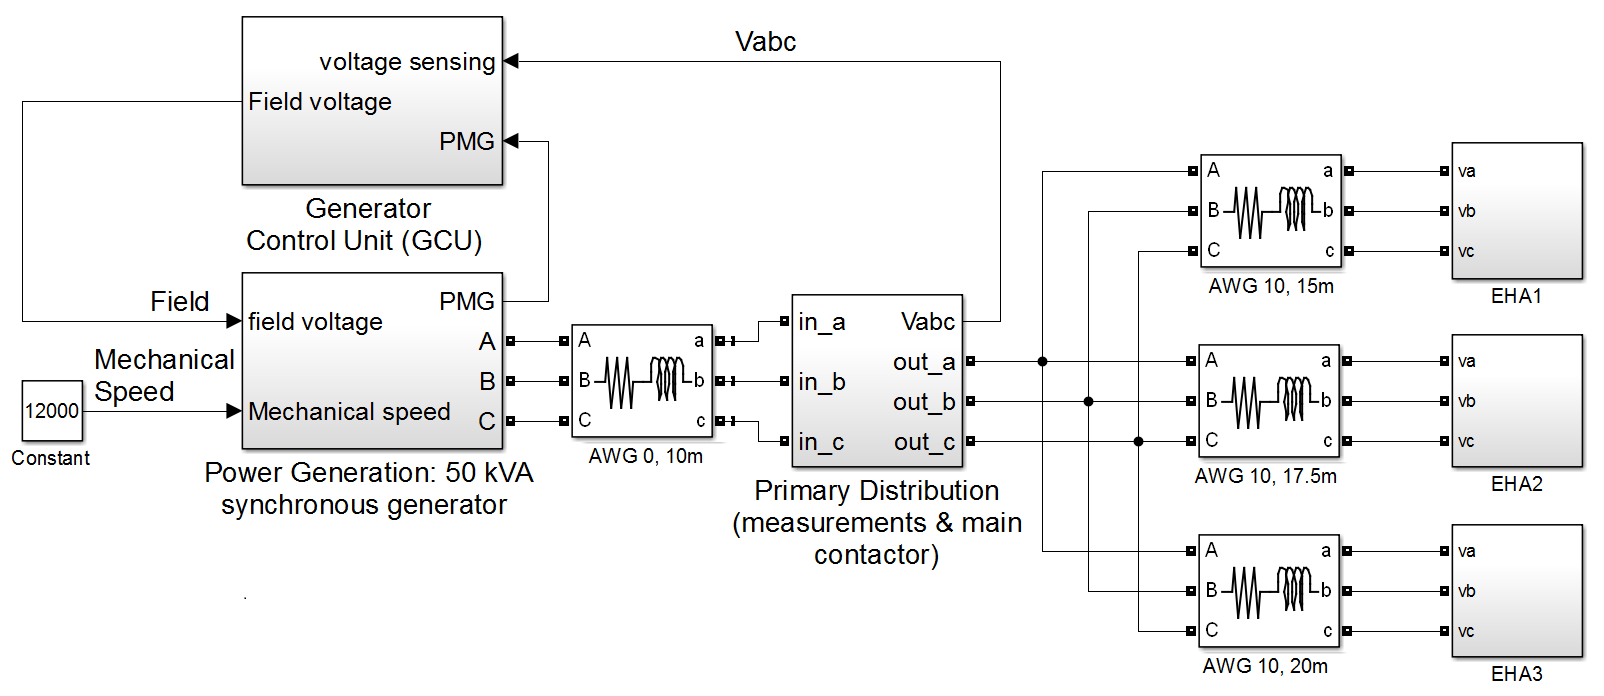
\includegraphics[width=0.6\textwidth]{Figures/simulacao_simulink.png}
	\caption{Electrical generation and distribution model}
	\label{fig:simulacao_simulink.png}
\end{figure*}

\subsection{Results}

The simulation results show the voltages and currents waveforms measured in the PCC, the voltage frequency spectrum, the amplitude constraints defined by the MIL-STD 704F, and the calculated value of the voltage THD and IHC.

The test is divided in two conditions:  the EHAs without operating and the EHAs starting their operation (maximum load). The results also show the cases where the active filters are connected and disconnected from the EHAs power input.

Fig. \ref{fig:artigo_unfilt_1.eps} and Fig. \ref{fig:artigo_unfilt_2.eps} show the system waveforms without active filters in the EHAs power inputs, when the EHAs are not in operation. Fig. \ref{fig:artigo_filt_1.eps} and Fig. \ref{fig:artigo_filt_2.eps} show the waveforms with the active filters connected to the EHAs power input for the same period. The active filters degrade the power quality during this time interval, since the THD increases and the frequency spectrum presents more harmonic content. This noise inserted in the system is due to the commutation of the VSC switching devices. Thus, even with the presence of the capacitor filter in the lines, some high frequency content injected in the grid was observed. However, the results are inside the limits defined by aeronautical standards.

Fig. \ref{fig:artigo_unfilt_3.eps} and Fig. \ref{fig:artigo_unfilt_4.eps} show the system waveforms without active filters connected to the grid, with the EHAs requiring maximum current. In the same time interval, Fig. \ref{fig:artigo_filt_3.eps} and Fig. \ref{fig:artigo_filt_4.eps} show the waveforms with the active filters connected to the EHAs power input. During this interval, it is clear the active filter enhancement in the system power quality. Considering these results, the active filter mitigates the harmonic content and set it within the limits of the MIL-STD 704F.

\begin{figure}[!h] %
	\centering
	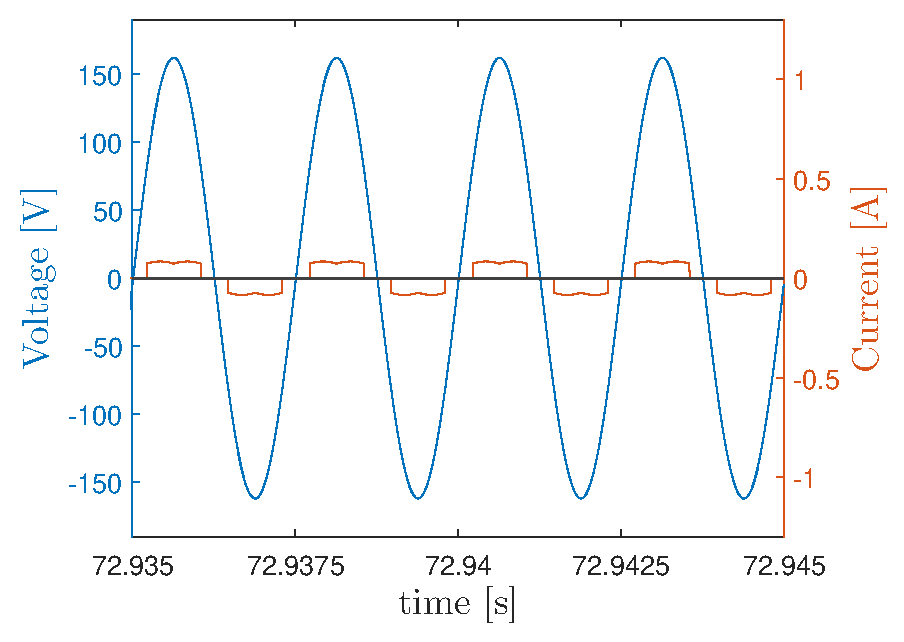
\includegraphics[width=0.27\textheight]{Figures/artigo_unfilt_1.eps}
	\caption{Voltage and current waveforms for the system without load and filter}
	\label{fig:artigo_unfilt_1.eps}
\end{figure}

\begin{figure}[!h] %
	\centering
	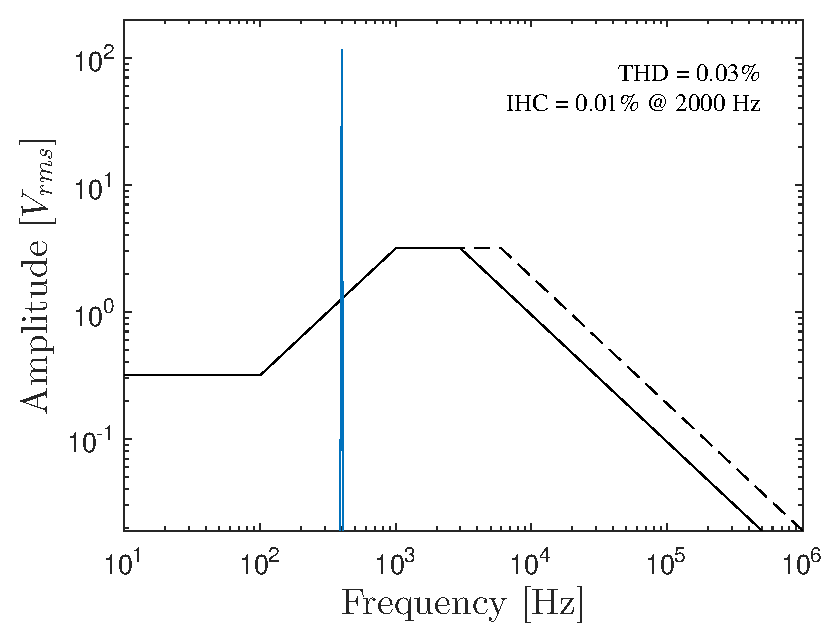
\includegraphics[width=0.27\textheight]{Figures/artigo_unfilt_2.eps}
	\caption{Voltage spectrum for the system without load and filter}
	\label{fig:artigo_unfilt_2.eps}
\end{figure}

\begin{figure}[!h] %
	\centering
	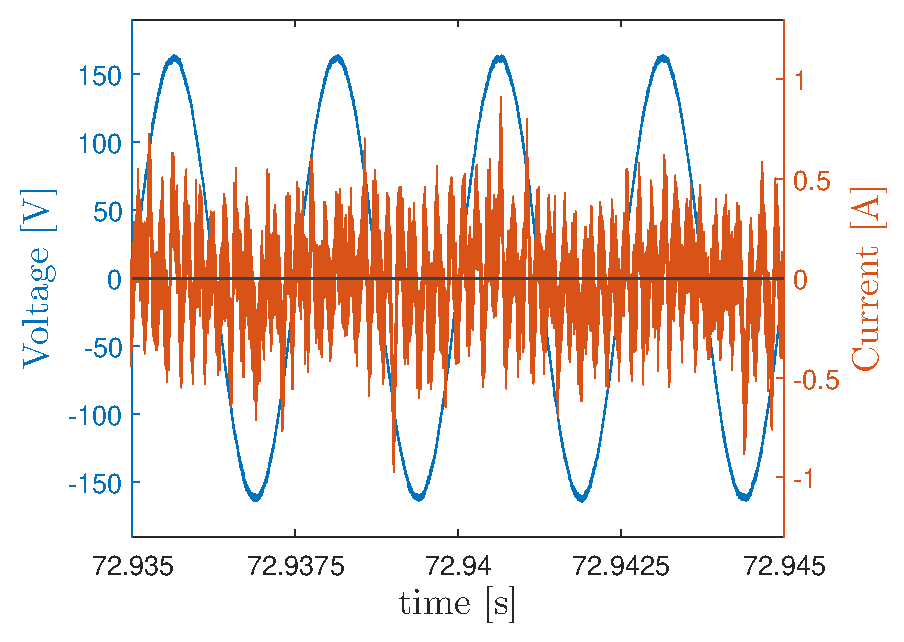
\includegraphics[width=0.27\textheight]{Figures/artigo_filt_1.eps}
	\caption{Voltage and current waveforms for the system without load and with filter}
	\label{fig:artigo_filt_1.eps}
\end{figure}

\begin{figure}[!h] %
	\centering
	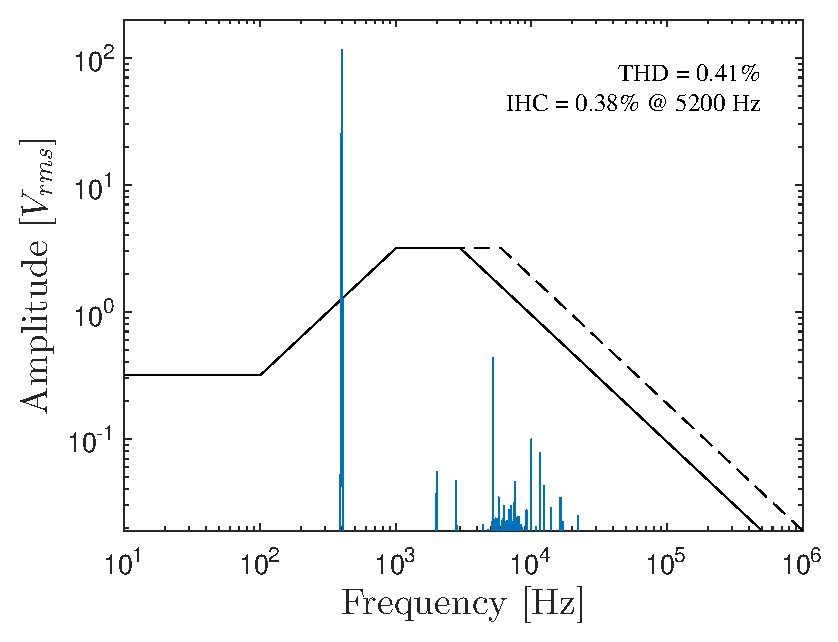
\includegraphics[width=0.27\textheight]{Figures/artigo_filt_2.eps}
	\caption{Voltage spectrum for the system without load and with filter}
	\label{fig:artigo_filt_2.eps}
\end{figure}

\begin{figure}[!h] %
	\centering
	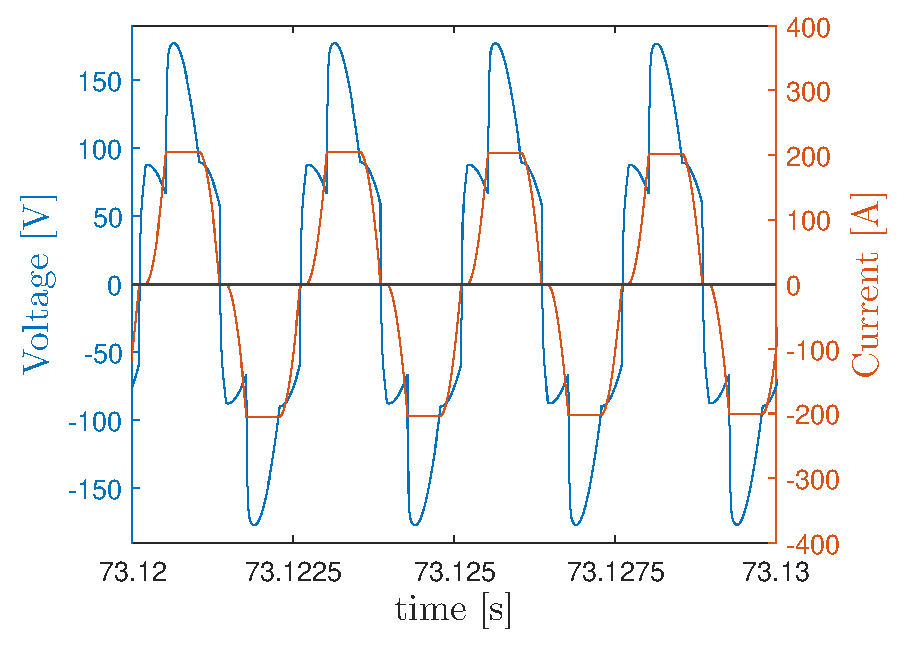
\includegraphics[width=0.27\textheight]{Figures/artigo_unfilt_3.eps}
	\caption{Voltage and current waveforms for the system with load and without filter}
	\label{fig:artigo_unfilt_3.eps}
\end{figure}

\begin{figure}[!h] %
	\centering
	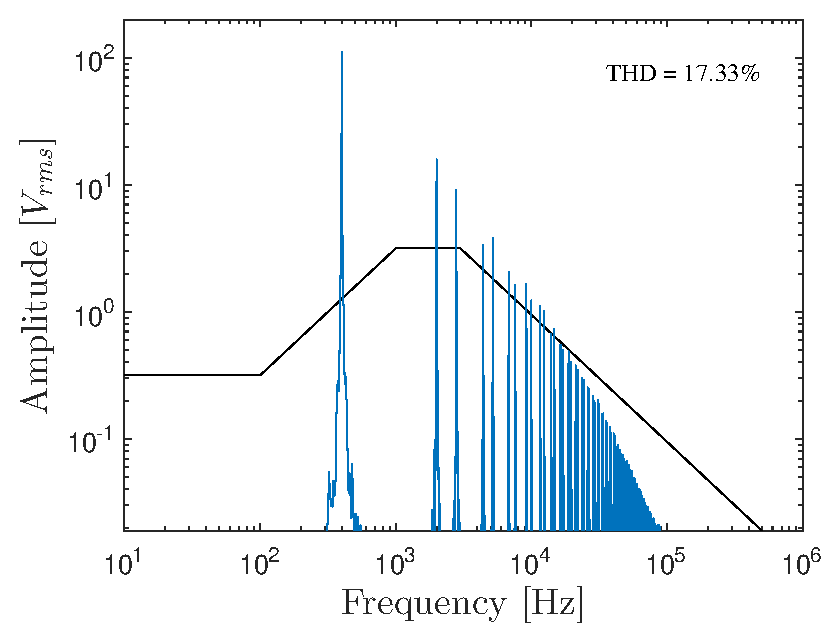
\includegraphics[width=0.27\textheight]{Figures/artigo_unfilt_4.eps}
	\caption{Voltage spectrum for the system with load and without filter}
	\label{fig:artigo_unfilt_4.eps}
\end{figure}

\begin{figure}[!h] %
	\centering
	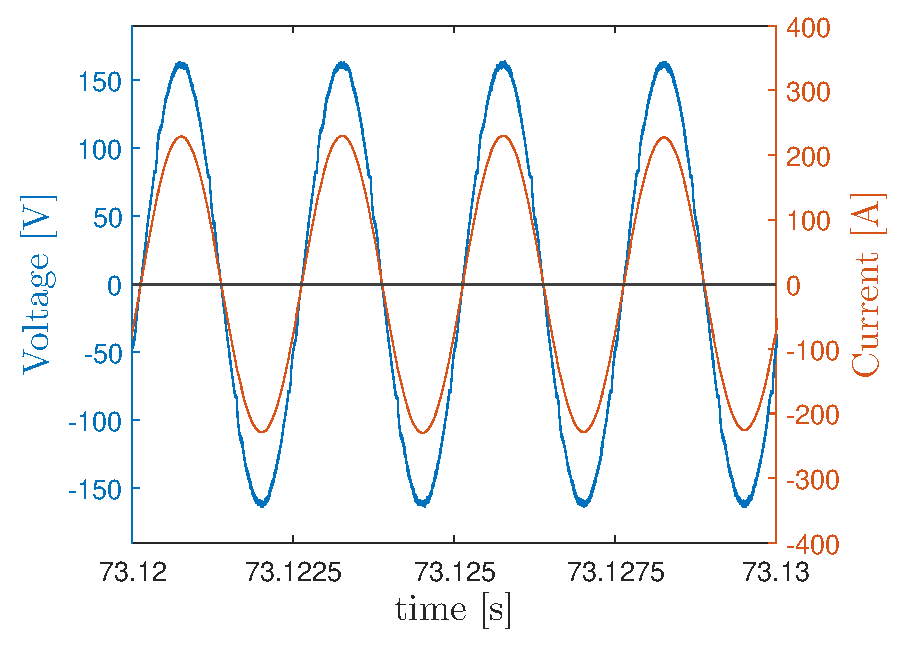
\includegraphics[width=0.27\textheight]{Figures/artigo_filt_3.eps}
	\caption{Voltage and current waveforms for the system with load and filter}
	\label{fig:artigo_filt_3.eps}
\end{figure}

\begin{figure}[!h] %
	\centering
	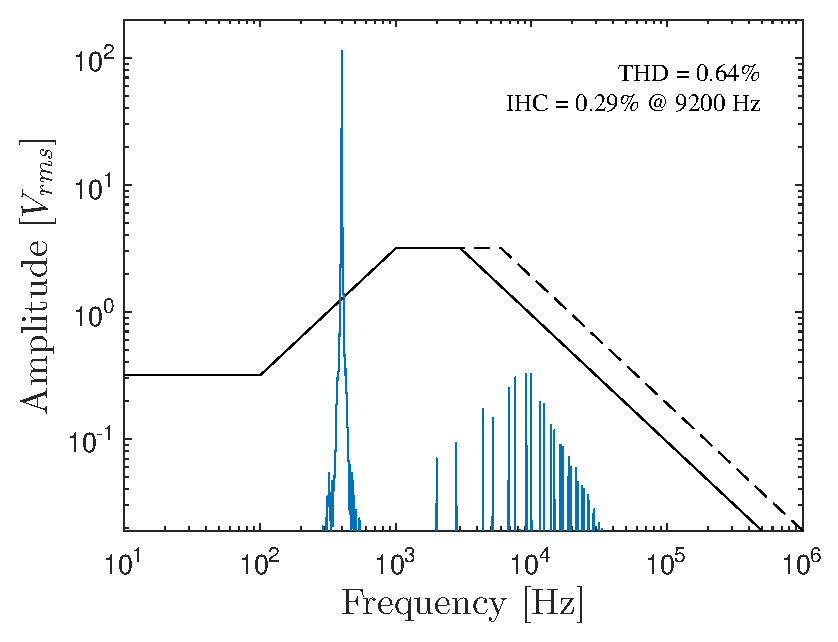
\includegraphics[width=0.27\textheight]{Figures/artigo_filt_4.eps}
	\caption{Voltage spectrum for the system with load and filter}
	\label{fig:artigo_filt_4.eps}
\end{figure}
\newpage
\section{Conclusions}

\todo[inline]{sintetizar uma breve conclusão derivada da dissertação}

Com base em tudo que foi escrito, enfatize a sua contribuição sem exageros.
Trabalhos futuros, deixe-os para um outro artigo. Concentre-se no que foi realizado.

\todo[inline]{Traduzir as Figuras}


%Introdução
%=============================================================================================
%\section{INTRODUÇÃO}
%  O texto da introdução deverá apresentar o contexto em que o artigo está inserido, seus objetivos e suas justificativas.
%	O Artigo\footnote{\scriptsize{Mais informações sobre a estruturação dos artigos estão contidas no site: \textcolor[rgb]{0,0,1}{http://eng.embraer.com.br/SETI/SETI/01.html-website/submissao\_artigos.html}.}} deve ser escrito em no máximo 25 páginas, incluindo Texto, Tabelas e/ou Figuras. 
%	A formatação deve seguir tamanho do papel A4, espaçamento entre linhas Simples, formatação do texto Justificado e margens superior, esquerda e direita de 25 mm e inferior 20 mm  (conforme modelo).
%	A língua oficial do congresso é o Português, entretanto serão aceitos artigos em Inglês. Porém, as apresentações deverão ser realizadas em Português. 
%	Os artigos devem ser rigorosamente formatados de acordo com estas instruções.
%
%%Metodologia
%%=============================================================================================
%\section{METODOLOGIA}
%Indicar sucintamente a metodologia utilizada no desenvolvimento do artigo.
%
%%Resultados
%%=============================================================================================
%\section{RESULTADOS}
%Apresentar os principais resultados obtidos no trabalho, podendo ser utilizados gráficos, tabelas e outras ilustrações necessárias à compreensão do tema.
%As equações devem ser apresentadas conforme mostrado pelas Equações \ \ref{e:newton} e \ \ref{e:eq2}.
%
%\begin{equation}
%		\label{e:newton}
%		F=m\alpha
%\end{equation}
%
%\begin{equation}
%		\label{e:eq2} % Este label sera usado para referenciar a equação em algum(s) ponto(s) do texto
%		B=\mu_{0}.(H+M)	
%\end{equation}
%
%As figuras devem ser referenciadas seqüencialmente na parte inferior das mesmas, seguidas do título e centralizadas, como mostrado na Figura \ \ref{figuraAEIOU}. É importante que a figura esteja legível. 
%
%\begin{figure}[htbp!]
%		\centering
%		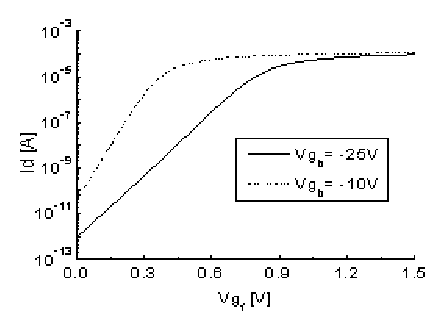
\includegraphics[width=0.5\textwidth]{./figs/Figura1.eps}
%		\caption{Título}
%		\label{figuraAEIOU}	% Usado para referenciar a figura em algum(s) ponto(s) do texto
%\end{figure}
%
%As tabelas devem ser referenciadas seqüencialmente na parte superior das mesmas, seguidas do titulo, como mostrado na Tabela \ \ref{tabelaUOIEA}. O texto da mesma deve ser centralizado.
%
%\begin{table}
%		\centering
%		\begin{tabular}{|c|c|c|c|}\hline
%							& Flaps & Actual & Stage 3 \\ 
%							& Setting & Noise Levels & (EPNdB)  \\
%							&         & (EPNdB)      &          \\ \hline
%			Flyover & 1 & 83.6  & 89.2 \\ \hline
%			Lateral & 1 & 92.6  & 95.3 \\ \hline
%			Approach & 6 & 92.5  & 99.2 \\ \hline
%		\end{tabular}
%		\caption{Título}
%		\label{tabelaUOIEA}
%\end{table}

%Comentários e Conclusões
%%=============================================================================================
%\section{COMENTÁRIOS E CONCLUSÕES}
%Destacar as principais contribuições do autor e indicar, de forma objetiva, as conclusões obtidas.
%
%\vspace{\baselineskip} % Comando para saltar linha (não precisa ter no Artigo final)
%\vspace{\baselineskip} % Comando para saltar linha (não precisa ter no Artigo final)
%
%\underline{\textbf{Referências:}}As referências devem ser indicadas ao longo do texto no formato Schutz (1997) ou (SCHUTZ, 1997) e descritas no final do artigo. Devem ser listados apenas os artigos mencionados no texto, em ordem alfabética do sobrenome, pelo primeiro autor. 
%
%A ordem dos itens em cada referência deve obedecer aos exemplos a seguir.
%\underline{Exemplos:}


%Referências bibliográficas
%=============================================================================================
\clearpage %Para que a parte das referências comece em uma nova página
%\bibliographystyle{apalike}

 \bibliographystyle{abbrvnat}
 \bibliography{Parts/bibliography}
%\setcitestyle{authoryear,open={((},close={))}}
 
%\begin{thebibliography}{50}% maximum number of references (for label width)
%			\bibitem{schutz:1997} SCHUTZ, E. \textbf{Reengenharia mental: reeducação de hábitos e programação de metas}. Florianópolis: Insular, 1997. ({\textbf{Exemplo de livro}})
%			\bibitem{williams:1950} WILLIAMS, J. W. \textbf{Flow measurement}. In: ROUSE, H. (org.). \textbf{Engineering hydraulics.}. New York: John Wiley \& Sons, 1950. p. 229-309. ({\textbf{Exemplo de capítulo de livro}})
%			\bibitem{cup:2003} CIENCIA E OPINIAO. Curitiba: Centro Universitário Positivo. 2003. ({\textbf{Exemplo de periódico}})
%			\bibitem{tozzi:2004} TOZZI, M.; OTA, J.  \textbf{Vertedouro em degraus}. Revista da Vinci, Curitiba, v.1, n.1, p. 9-28, 2004. ({\textbf{Exemplo de artigo de periódico}})
%			\bibitem{veiga:2001} VEIGA, B. V.  \textbf{Modelagem computacional do processo de eutrofização de aplicação de um modelo de balanço de nutrientes a reservatórios da região metropolitana de Curitiba}. Curitiba, 140 p., 2001. Dissertação (Mestrado) – Universidade Federal do Paraná. ({\textbf{Exemplo de monografia, dissertação e tese}})
%			\bibitem{arcdesign:2004} ARC DESIGN. \textbf{Mestres da Arquitetura:} Oscar Niemeyer. São Paulo: Quadrifoglio, n. 35, mar. - abril, 2004. ({\textbf{Exemplo de publicações periódicas consideradas em parte (suplementos, fascículos, números especiais) }})
%			\bibitem{moreira:2004} MOREIRA, T. \textbf{Debate sobre software livre chega ao celular}. Valor Econômico, São Paulo, 04 out. 2004. p. B4. ({\textbf{Exemplo de artigo de jornal}})
%			\bibitem{yoshida:1996} YOSHIDA, S.; VENDRAMIN, J.C.; OLIVEIRA C. \textbf{Tratamento térmico em matrizes de forjaria em prensas de martelo: como aumentar a vida útil}. In: SEMINÁRIO NACIONAL DE FORJAMENTO, 16., Porto Alegre. Anais... Porto Alegre: UFRGS – Centro de Tecnologia, 1996. p. 29-39 ({\textbf{Exemplo de artigo de jornal}})
%			\bibitem{moura:2009} MOURA, G. C. de M. Citação de referências e documentos eletrônicos. Disponível em: \textcolor[rgb]{0,0,1}{http://www.elogica.com.br/users/gmoura/refere.html} Acesso em: 07/01/2009 as 14:00hs. ({\textbf{Exemplo de internet}})
%\end{thebibliography}



\end{document}

